\documentclass[10pt,a4paper]{article}
\usepackage[utf8]{inputenc}
\usepackage{amsmath}
\usepackage{amsfonts}
\usepackage{amssymb}
\usepackage[]{algorithm2e}
\usepackage{graphicx}
\usepackage[left=2cm,right=2cm,top=2cm,bottom=2cm]{geometry}

\begin{document}

\title{LINGI2261: Artificial Intelligence \\
Assignement 3 : Adversarial Search}
\author{Group 8: Ndizera Eddy \and El Jilali Solaiman}
\date{\today}
\maketitle

\section{Alpha-Beta search}

\subsection{Perform the MiniMax algorithm on the tree in Figure 1, i.e. put a value to each node. Circle the move the root player should do.}

\begin{figure}[h]
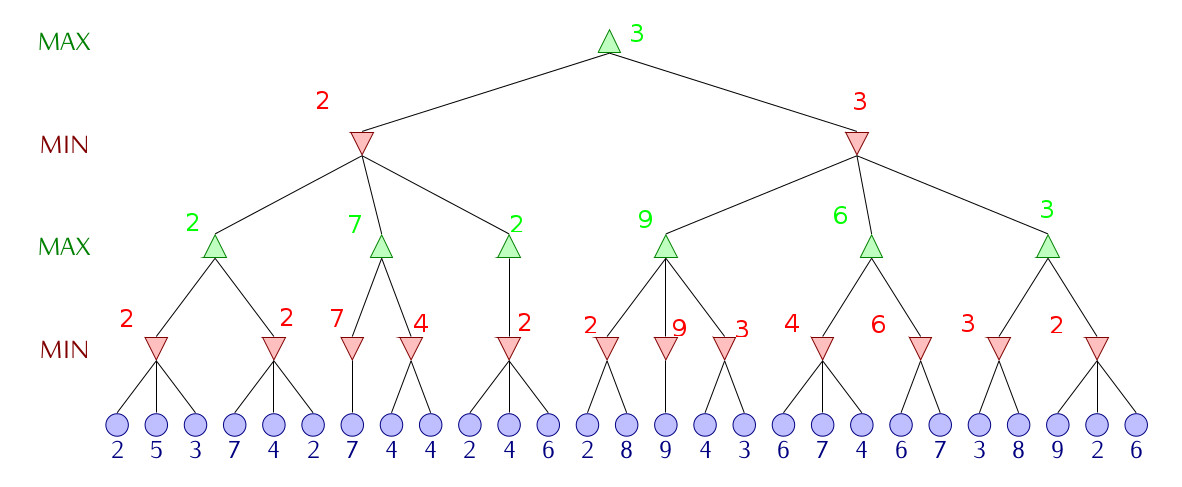
\includegraphics[scale=0.4]{img/minimax.jpg} 
\caption{\label{minimax} MiniMax}
\end{figure}

\subsection{Perform the Alpha-Beta algorithm on the tree in Figure 2. At each non terminal node, put the successive values of $ \alpha $ and $ \beta $. Cross out the arcs reaching non visited nodes. Assume a left-to-right node expansion.}

\begin{figure}[h]
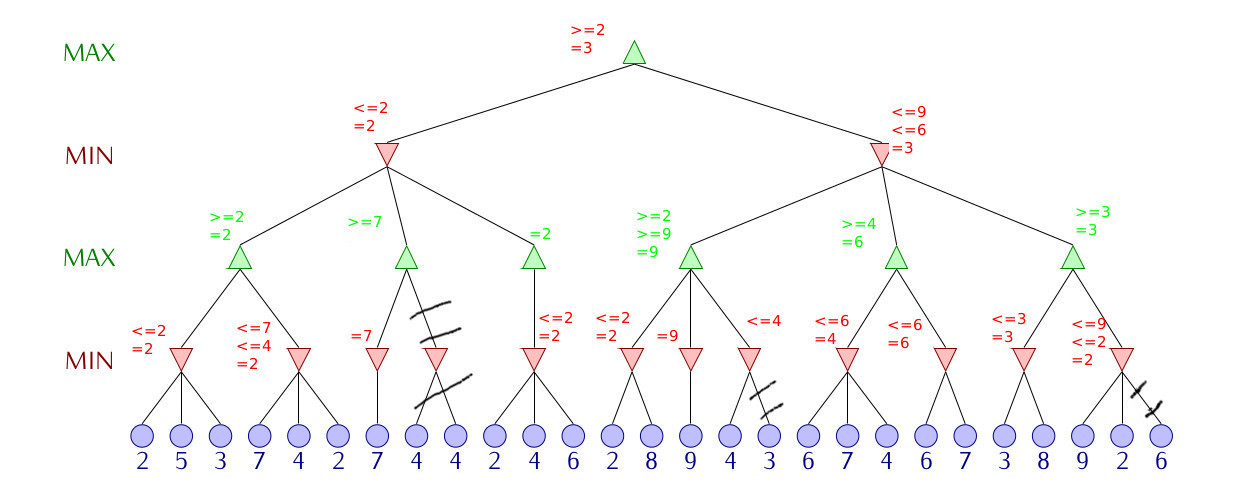
\includegraphics[scale=0.4]{img/alphabeta_left.jpg} 
\caption{\label{alphabetaleft} Alpha-Beta, left-to-right expansion}
\end{figure}

\subsection{Do the same, assuming a right-to-left node expansion instead (Figure 3).}

\begin{figure}[h]
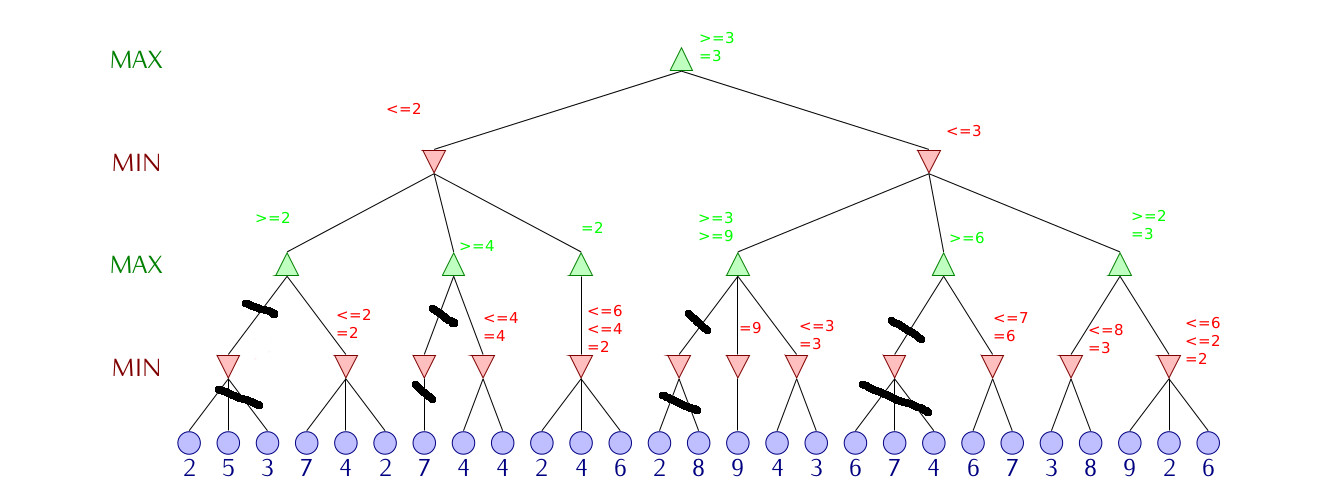
\includegraphics[scale=0.4]{img/alphabeta_right.jpg} 
\caption{\label{alphabetaright} Alpha-Beta, right-to-left expansion}
\end{figure}

\subsection{Can the nodes be ordered in such a way that Alpha-Beta pruning can cut off more branches (in a left-to right node expansion)? If no, explain why; if yes, give the new ordering and the resulting new pruning.}

Yes, if we order the nodes in increasing order like shown in Figure \ref{alphabetanodes}, the Alpha-Beta pruning will cut off more branches. The nodes must be set in that order because it's MIN that chooses the action to pick in the bottom of the tree.
%The idea is to first examine the best node at each depth (Min or Max) \\
%\begin{itemize}
%	\item For max nodes, we want to visit the best child first so that time is not wasted in the rest of the children exploring worse scenarios.
%	\item For min nodes, we want to visit the worst child first
%\end{itemize}
%If we reorder all the tree in that way, we can pass more childrens nodes because at the parent level all those childrens nodes will imply a cutoff.


\begin{figure}[h]
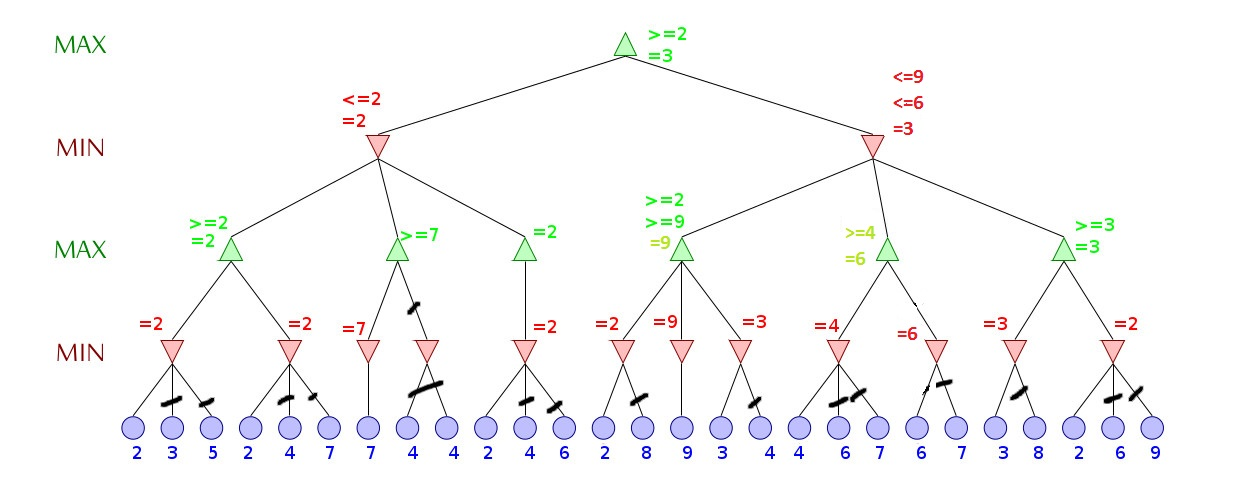
\includegraphics[scale=0.4]{img/alphabeta_nodes.jpg} 
\caption{\label{alphabetanodes} Alpha-Beta, left-to-right expansion}
\end{figure}

\section{Avalam}

\subsection{A basic Alpha-Beta Agent}

The basic Alpha-Beta Agent can be found on INGInious.

\subsection{Comparison of two evalutaion functions}

\subsubsection{Launch a game where one of the agents is the basic agent described before against another agent where the basic evaluate method has been replaced such that it returns directly the result of Board.get\_score instead of -1, 0 or 1. Watch the replay of the match. What do you observe? Does one of the agent clearly overcomes the other one? Explain why there is such a difference.}

A first observation is that the player to play first is the one winning the game. But a second observation is that the agent with it's evaluation function equals to the Board.get\_score method is the one winning with a greater margin. The reason that this agent wins with a higher margin is that it's evaluation function returns values different than 0, 1 or -1. Thus, it can describes  losing states that are, for example, more disadvantageous for him whereas the other one will classify all the losing states as the same.


\subsection{Describe precisely your evaluation function.}
Our conception of the evaluation function cames from a simple observation. If a player has a tower of height three surrounded by at least two opponents tower of height one, the opponent has a very high probability to complete a tower. By that we mean a tower of height five. Thus we avoid to have a situation where we have a tower of height three surrounded by two opponent towers of height one but we try to have the opposite situation where we surround opponents tower of height three by at least two of our tower of height one. \\

Our evaluate function returns then the difference between opponents towers of height three surrounded and our towers of height three surrounded. This is done in case the two players have the same score. By the score we mean the number of towers owned. We calculate the numbers of towers surrounded after the score because if we had chosen the inverse order, our agent would consider some situations positives because he surrounds a lot of towers of height three, but in reality the score is in advantage of the opponent player.\\

At last, if the score and the number of towers surrounded are the same for the two players, we consider the difference of towers of height five for the two players to determine the value of the state. \\

The fig.\ref{evaluation} illustrates the advantage created by our evaluation function.
In most case, the blue player has the advantage. If player red put his tower of height three on top of one of the other counter, the red player can form a tower of height five. If he moves one of it's counter (height one) on another counter, we can form another tower of height three.\\

\begin{figure}[h]
\center
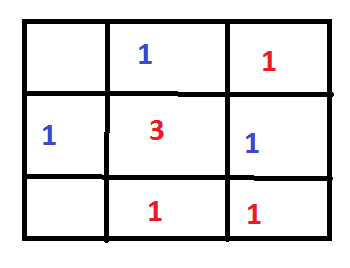
\includegraphics[scale=0.4]{img/evaluation.png} 
\caption{\label{evaluation} Tower of three surrounded}
\end{figure}


In summmary, our evaluate function, calculate first the difference of score, then if it's null, the difference of towers of height three surrounded and finally, if the two are null, the difference of towers of height five.

\subsection{Give an upper and a lower bound on the branching factor for a search tree on the Avalam game. Justify your answer.}

An upper bond for the branching factor could be 48*8=\textbf{384}. The number \textit{48} represents the number of counters at the beginning of the game. Each of these counters can be moved in \textit{8} directions (we put an upper bond by supposing that the towers on the borders can move in 8 directions). By multiplicating these two numbers we obtain the number of moves we can do at the beginning of the game which is the upper bound for the branching factor. \\

Thus a lower bound would be \textbf{2}, which represents the fact that we can only move two towers (or counters) towards each other. This is due to the fact that if we can move a tower towards another one then the reciprocal can be done also.\\

We can then say that the branching factor is comprise in the interval \textbf{[384, 2]}.

\subsection{How does the branching factor evolve after a move has been performed? Explain.}

The branching factor decreases after a move has been performed. If we move a counter (or tower) on another counter (or tower), then the number of possible moves decreases by a minimum value of 2 which is the possibility for counter A to move on counter B and the reciprocal. Also by moving a counter or tower we obtain fewer counters and towers on the board. Thus there is fewer possibilities for counters to be moved because the number of empty spaces increase and there are other situations that limits the possibility to move like for example it's not permitted to put a tower of height 2 on a tower of height 4. \\

In conclusion, the branching factor decreases as the number of moves increases.

\subsection{Can you think of states that might be ignored? What do you loose if you ignore successors? Explain.}

States that can be ignored are the one where we decrease our score. As this game is essentially about decreasing the score of the opponent, using a turn to decrease our score is not a good idea as a difference of even two points in this game is huge. So the states that we considered to be ignored are the following ones:

\begin{itemize}
\item Put an opponent tower on one of our tower
\item One of our tower on another of our tower. This action should only be done at end of the game when we don't have the choice.
\end{itemize}

We found other states that can be ignored because they lead to bad situations:

\begin{itemize}
\item Give a tower to the opponent (fig.\ref{states_ignored}). That case can occur by forming a tower of height five for the opponent, or forming a tower with opponent counter at top and we don't have the possibility to regain that tower. By that we mean that the tower cannot be moved (for example if the tower become isolated).
\item Create a tower of height $x$ next to a tower of height $5-x$ with a different color in the neighborhood. This is a very bad situation where the opponent can exploit that to create directly a tower of height five. 
\end{itemize}

\begin{figure}[h]
\center
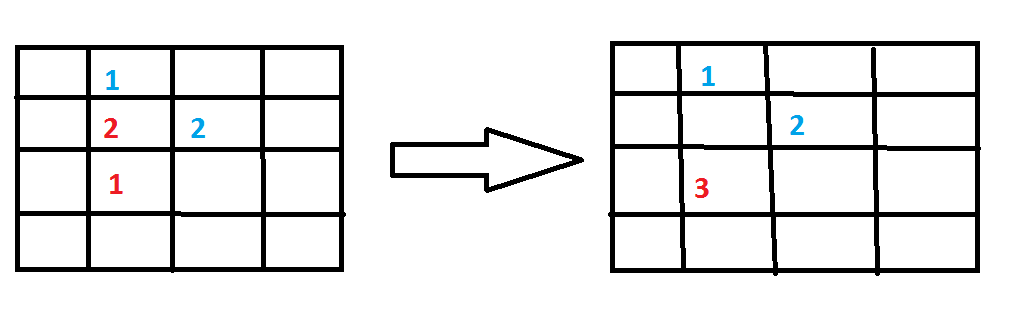
\includegraphics[scale=0.4]{img/states_ignored.png} 
\caption{\label{states_ignored} Give a tower to an opponent}
\end{figure}

But we also found a state that should be exploited at all cost. If we have a tower of height $x$ next to a tower of height $5-x$ with the opponent color, we have to put our tower on top of the opposite tower. This situation is great because we decrease the opponent's score by one and we create a tower of height five which is a point that cannot be contested. \\

By ignoring states, we decrease the branching factor interval which is [384, 2] to [192, 2]. This allows us to compute faster a search tree and also to go deeper in the search. However by ignoring states a problem arise at the end of the game where all moves possibles are considered not good and therefore ignored. So there should be a special case as when all the moves are all considered ignored, expand them. Also by ignoring states, it's obvious that we consider the opponent to be as smart as us which don't always hold true. 

\subsection{Describe your successors function.}

As explained earlier, in our successors function we first search for an action that could create a tower of height five by placing our tower (of height $x$) on top of an opponent's tower (of height $5-x$). The search is done by looking for towers of height three and four ( as we can have five in two ways, 4+1 and 3+2) and checking for those towers if a complementary tower (for three it's two and for four it's one) of opposite color is next to them. If an action is found that permits to create a tower of height five, we only return the state that is a result of that action. We force the agent to play that action.\\

If the search is negative, we consider all the actions possible and only returns the ones we consider to be good based on a function that check if a new state is considered good to play or not as explained in the previous question. But when the game is close to it's end, generally all the moves possibles are considered not good by our funtion. Therefore if we don't find a good move to do, we return all the bad actions. But like said, it happens generally at the end of the game.


\subsection{The cutoff method receives an argument called depth. Explain precisely what is called the depth in the minimax.py implementation.}

The argument depth is the number of actions to obtain the current state given an initial state. If we represents the minimax as a tree. The root's node is the initial state and the edges are the actions to obtain the current node/state.

\subsection{Explain why it might be useful (for the Avalam contest) to cut off the search for another reason than the depth. Would it be interesting to consider a changing cutoff function (i.e. it changes according to the advancement of the game).}

The time could influence the cut-off function in the sense that we have to share time slices between all turns. Because the branching factor is higher at the beginning of the game, it's more accurate to allocate more time at the beginning and less at the end. Also it could be interesting to take more time by search in a game of twenty minutes than a game of 5 minutes , thus increasing the depth limit of the search. We could then create a cut-off function that assign a default time limit by search which is equal to the time of the game divided by the number of turn of a typical game which is roughly forty. From that we can create improvements like adding more time to the searchs occuring at the beginning of the game or taking into account the time remaining and decreasing the default time limit or increasing it.\\

The step number also (which is the number of turns played) can also influence the cut-off function because higher is the step number, less are the possibilities. This is due to the fact that the branching factor decreases after each move like explained before. A smaller branching factor permits to search deeper in the tree. With that we can create a cut off function that assigns a maximum depth for a range of step numbers in a way higher is the step number, higher is the depth.\\

With the step numbers or time, we can, like explained, create a changing, dynamic cut-off function that adapts according to the advancement of the game.

\subsection{Describe your cut-off function.}

For our cut-off function, we chose to consider the step number to determine the maximum depth of the search. We increase the maximum depth proportionally to the step number. Basically, we assign a maximum depth for a range of step numbers so as greater is the range, greater is the maximum depth. \\

Also we make sure to have a maximum depth which is odd (last action is done by our agent) as it gives us better performance. With our implementation, it is better to apply our evaluation function on a state which is done by us. This holds mainly true if we play second. Because by moving a tower we will restore the equality of the score, our evaluation function will then emphasize the fact that we surround tower of height three or not.

\subsection{Describe concisely your super tough agent in your report. Your description shouldn’t be longer than one A4 paper page; if it is the same agent than the one described in earlier sections, just state it, no need to re-explain.}

Our \textit{super\_agent} is the same as our \textit{contest\_agent}. All the above description are therefore the same for our \textit{contest\_agent}.

\end{document}
